%-----------------------------------------------------------------------------%
\chapter{\babTiga}


%-----------------------------------------------------------------------------%
\lipsum[6-6]

%-----------------------------------------------------------------------------%
\section{Kedudukan dan Koordinasi}
%-----------------------------------------------------------------------------%


\lipsum[7-8]

\noindent \begin{align}\label{eq:garis}
	\cfrac{y - y_{1}}{y_{2} - y_{1}} = 
	\cfrac{x - x_{1}}{x_{2} - x_{1}}
\end{align}

\equ~\ref{eq:garis} di atas adalah persamaan garis. 
\equ~\ref{eq:garis} dan \ref{eq:bola} sama-sama dibuat dengan perintah \bslash
align. 
Perintah ini juga dapat digunakan untuk menulis lebih dari satu persamaan. 

\noindent \begin{align}\label{eq:bola}
	\underbrace{|\overline{ab}|}_{\text{pada bola $|\overline{ab}| = r$}} 
		= \sqrt[2]{(x_{b} - x_{a})^{2} + (y_{b} - y_{a})^{2} + 
				\vert\vert(z_{b} - z_{a})^{2}}
\end{align}

%-----------------------------------------------------------------------------%
\section{Tugas yang Dilakukan}
\label{sec:multiEqu}
%-----------------------------------------------------------------------------%

\lipsum[9-10]

% %-----------------------------------------------------------------------------%
% \section{Membuat Tabel}
% %-----------------------------------------------------------------------------%
% Seperti pada gambar, tabel juga dapat diberi label dan caption. 
% Caption pada tabel terletak pada bagian atas tabel. 
% Contoh tabel sederhana dapat dilihat pada \tab~\ref{tab:tab1}.

\begin{table}
	\centering
	\caption{Contoh Tabel}
	\label{tab:tab1}
	\begin{tabular}{l | c r}
		\hline
		& kol 1 & kol 2 \\ 
		\hline
		baris 1 & 1 & 2 \\
		baris 2 & 3 & 4 \\
		baris 3 & 5 & 6 \\
		jumlah  & 9 & 12 \\
		\hline
	\end{tabular}
\end{table}

Ada jenis tabel lain yang dapat dibuat dengan \latex~berikut 
beberapa di antaranya. 
Contoh-contoh ini bersumber dari 
\url{http://en.wikibooks.org/wiki/LaTeX/Tables}

\begin{table}
	\centering
	\caption{An example of rows spanning multiple columns}
	\label{row.spanning}
	\begin{tabular}{l l *{6}{c}}
  		\hline % create horizontal line
  		No & Name & \multicolumn{3}{c}{Week 1} & \multicolumn{3}{c}{Week 2} \\
  		\cline{3-8} % create line from 3rd column till 8th column
  		& & A & B & C & A & B & C\\
  		\hline
  		1 & Lala & 1 & 2 & 3 & 4 & 5 & 6\\
  		2 & Lili & 1 & 2 & 3 & 4 & 5 & 6\\
  		3 & Lulu & 1 & 2 & 3 & 4 & 5 & 6\\
  		\hline
	\end{tabular}
\end{table}

\lipsum[43-44]

\begin{table}
	\centering
	\caption{Penulisan judul tabel dan judul gambar adalah rata kiri kanan serta tidak dicetak tebal dan mengikuti cara penulisan kalimat (sentence case).}
	\label{column.spanning}
	\begin{tabular}{l c l}
		\hline
		Percobaan & Iterasi & Waktu \\
		\hline
		Pertama & 1 & 0.1 sec \\ \hline
		\multirow{2}{*}{Kedua} & 1 & 0.1 sec \\
 		& 3 & 0.15 sec \\ 
 		\hline
		\multirow{3}{*}{Ketiga} & 1 & 0.09 sec \\
 		& 2 & 0.16 sec \\
 		& 3 & 0.21 sec \\ 
 		\hline
	\end{tabular}\\
	\vspace{1em}
	{\small Sumber: \url{http://en.wikibooks.org/wiki/LaTeX/Tables}}
\end{table}


\lipsum[45-46]

\noindent \begin{align}\label{eq:matriks}	
	|\overline{a} * \overline{b}| &= |\overline{a}| |\overline{b}| \sin\theta 
		\\[0.2cm]
	\overline{a} * \overline{b} &=  
		\begin{array}{| c c c |}
			\hat{i} & x_{1} & x_{2} \\
			\hat{j} & y_{1} & y_{2} \\
			\hat{k} & z_{1} & z_{2} \\
		\end{array} \nonumber \\[0.2cm]
	&= \hat{i} \,
		\begin{array}{ | c c | }
			y_{1} & y_{2} \\
			z_{1} & z_{2} \\
		\end{array} 
	   + \hat{j} \,
		\begin{array}{ | c c | }
			z_{1} & z_{2} \\
			x_{1} & x_{2} \\
		\end{array} 
	   + \hat{k} \,	
		\begin{array}{ | c c | }
			x_{1} & x_{2} \\
			y_{1} & y_{2} \\
		\end{array}
		\nonumber
\end{align}

Pada \equ~\ref{eq:matriks} dapat dilihat beberapa baris menjadi satu bagian 
dari \equ~\ref{eq:matriks}. 
Sedangkan di bawah ini dapat dilihat bahwa dengan cara yang sama, \equ~
\ref{eq:gabungan1}, \ref{eq:gabungan2}, dan \ref{eq:gabungan3} memiliki nomor 
persamaannya masing-masing. 

\noindent \begin{align}\label{eq:gabungan1}	
	\int_{a}^{b} f(x)\, dx + \int_{b}^{c} f(x) \, dx = \int_{a}^{c} f(x) \, dx
		\\\label{eq:gabungan2}
	\lim_{x \to \infty} \frac{f(x)}{g(x)} = 0 \hspace{1cm} 
		\text{jika pangkat $f(x)$ $<$ pangkat $g(x)$} \\\label{eq:gabungan3}
	a^{m^{a \, ^{n}\log b }} = b^{\frac{m}{n}}
\end{align}



Rumus \ref{eq:Precision} menunjukkan cara perhintungan \textit{Precision}.

\addequation{\textit{Precision}}{%
\begin{equation}  \label{eq:Precision}
    Precision = \frac{TP}{TP+FP}
\end{equation}
}

Rumus \ref{eq:Recall} menunjukkan cara perhitungan \textit{Recall}.

\addequation{\textit{Recall}}{
\begin{equation}  \label{eq:Recall}
    Recall = \frac{TP}{TP+FN}
\end{equation}

}

\addequation{\textit{F1 Score}}{%
\begin{equation}  \label{eq:F1-score}
    F1 Score = 2*\frac{Precision*Recall}{Precision+Recall}
\end{equation}
}


\section{Uraian Pelaksanaan Magang}

\lipsum[34-35]

Pelaksanaan kerja magang diuraikan seperti pada Tabel \ref{tbl_uraian}.

\begin{table}
	\centering
	\caption{ Pekerjaan yang dilakukan tiap minggu selama pelaksanaan kerja magang}
	\label{tbl_uraian}
	\begin{tabular}{|c | p{0.75\textwidth}| }
		\hline
		Minggu Ke - & Pekerjaan yang dilakukan \\
		\hline
		1 & Memahami .... \\
		\hline
 		2 & Menerapkan desain UI/UX pada ..... \\
		\hline
 		3 & Menerapkan desain UI/UX untuk.....  \\
 		\hline
 		4 & Melakukan ...... \\
 		\hline
 		5 & Membuat ......... \\
 		\hline
 		6 & \\
 		\hline
	\end{tabular}
\end{table}


\subsection{Sub-section}

\lipsum[11-12]


\begin{figure}
     \centering
     \begin{subfigure}[b]{0.3\textwidth}
         \centering
         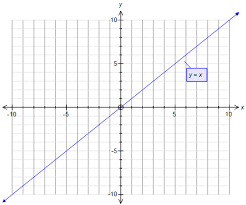
\includegraphics[width=\textwidth]{assets/pics/graph1.png}
         \caption{$y=x$}
         \label{fig:y equals x}
     \end{subfigure}
     \hfill
     \begin{subfigure}[b]{0.3\textwidth}
         \centering
         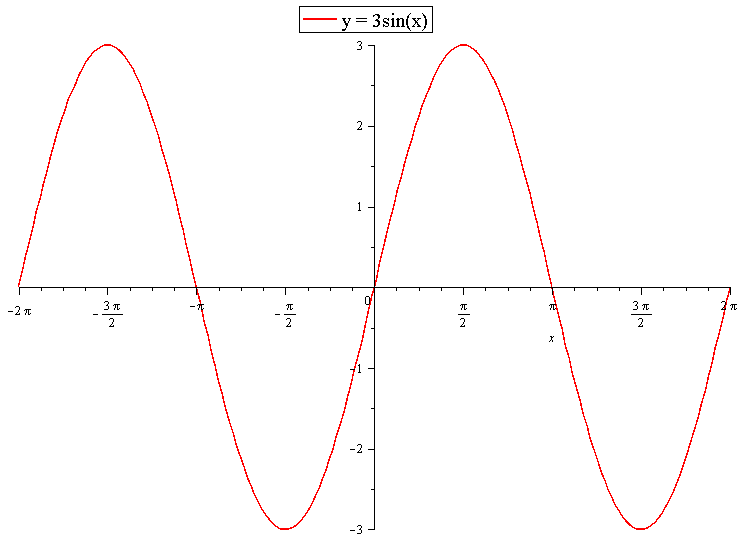
\includegraphics[width=\textwidth]{assets/pics/graph2.png}
         \caption{$y=3sinx$}
         \label{fig:three sin x}
     \end{subfigure}
     \hfill
     \begin{subfigure}[b]{0.3\textwidth}
         \centering
         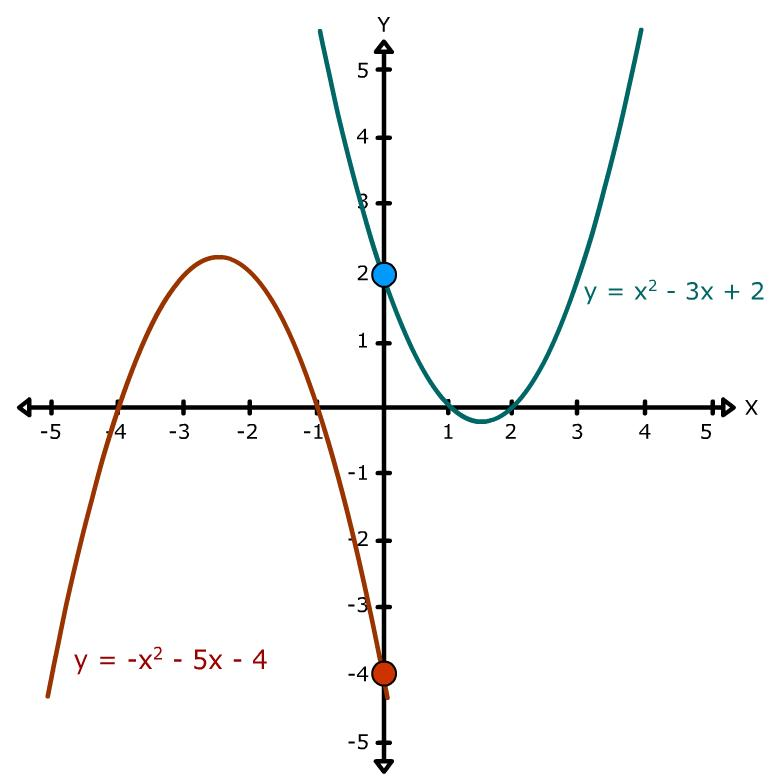
\includegraphics[width=\textwidth]{assets/pics/graph3.jpg}
         \caption{$y=5/x$}
         \label{fig:five over x}
     \end{subfigure}
        \caption{Three simple graphs}
        \label{fig:three graphs}
\end{figure}



\subsubsection{Subsub-section}

\lipsum[13-14]


\begin{center}
\begin{longtable}{|l|l|l|}
\caption{A sample long table} \label{tab:long} \\

\hline \multicolumn{1}{|c|}{\textbf{First column}} & \multicolumn{1}{c|}{\textbf{Second column}} & \multicolumn{1}{c|}{\textbf{Third column}} \\ \hline 
\endfirsthead

\multicolumn{3}{c}%
{{ \tablename\ \thetable{} \small A sample long table (lanjutan)}} \\
\hline \multicolumn{1}{|c|}{\textbf{First column}} & \multicolumn{1}{c|}{\textbf{Second column}} & \multicolumn{1}{c|}{\textbf{Third column}} \\ \hline 
\endhead

\hline \multicolumn{3}{|r|}{{Lanjut pada halaman berikutnya}} \\ \hline
\endfoot

\hline \hline
\endlastfoot

One & abcdef ghjijklmn & 123.456778 \\
One & abcdef ghjijklmn & 123.456778 \\
One & abcdef ghjijklmn & 123.456778 \\
One & abcdef ghjijklmn & 123.456778 \\
One & abcdef ghjijklmn & 123.456778 \\
One & abcdef ghjijklmn & 123.456778 \\
One & abcdef ghjijklmn & 123.456778 \\
One & abcdef ghjijklmn & 123.456778 \\
One & abcdef ghjijklmn & 123.456778 \\
One & abcdef ghjijklmn & 123.456778 \\
One & abcdef ghjijklmn & 123.456778 \\
One & abcdef ghjijklmn & 123.456778 \\
One & abcdef ghjijklmn & 123.456778 \\
One & abcdef ghjijklmn & 123.456778 \\
One & abcdef ghjijklmn & 123.456778 \\
One & abcdef ghjijklmn & 123.456778 \\
One & abcdef ghjijklmn & 123.456778 \\
One & abcdef ghjijklmn & 123.456778 \\
One & abcdef ghjijklmn & 123.456778 \\
One & abcdef ghjijklmn & 123.456778 \\
One & abcdef ghjijklmn & 123.456778 \\
One & abcdef ghjijklmn & 123.456778 \\
One & abcdef ghjijklmn & 123.456778 \\
One & abcdef ghjijklmn & 123.456778 \\
One & abcdef ghjijklmn & 123.456778 \\
One & abcdef ghjijklmn & 123.456778 \\
One & abcdef ghjijklmn & 123.456778 \\
One & abcdef ghjijklmn & 123.456778 \\
One & abcdef ghjijklmn & 123.456778 \\
One & abcdef ghjijklmn & 123.456778 \\
One & abcdef ghjijklmn & 123.456778 \\
One & abcdef ghjijklmn & 123.456778 \\
One & abcdef ghjijklmn & 123.456778 \\
One & abcdef ghjijklmn & 123.456778 \\
One & abcdef ghjijklmn & 123.456778 \\
One & abcdef ghjijklmn & 123.456778 \\
One & abcdef ghjijklmn & 123.456778 \\
One & abcdef ghjijklmn & 123.456778 \\
One & abcdef ghjijklmn & 123.456778 \\
One & abcdef ghjijklmn & 123.456778 \\
One & abcdef ghjijklmn & 123.456778 \\
One & abcdef ghjijklmn & 123.456778 \\
One & abcdef ghjijklmn & 123.456778 \\
One & abcdef ghjijklmn & 123.456778 \\
One & abcdef ghjijklmn & 123.456778 \\
One & abcdef ghjijklmn & 123.456778 \\
One & abcdef ghjijklmn & 123.456778 \\
One & abcdef ghjijklmn & 123.456778 \\
One & abcdef ghjijklmn & 123.456778 \\
One & abcdef ghjijklmn & 123.456778 \\
One & abcdef ghjijklmn & 123.456778 \\
One & abcdef ghjijklmn & 123.456778 \\
One & abcdef ghjijklmn & 123.456778 \\
One & abcdef ghjijklmn & 123.456778 \\
One & abcdef ghjijklmn & 123.456778 \\
One & abcdef ghjijklmn & 123.456778 \\
One & abcdef ghjijklmn & 123.456778 \\
One & abcdef ghjijklmn & 123.456778 \\
One & abcdef ghjijklmn & 123.456778 \\
One & abcdef ghjijklmn & 123.456778 \\
One & abcdef ghjijklmn & 123.456778 \\
One & abcdef ghjijklmn & 123.456778 \\
One & abcdef ghjijklmn & 123.456778 \\
One & abcdef ghjijklmn & 123.456778 \\
One & abcdef ghjijklmn & 123.456778 \\
One & abcdef ghjijklmn & 123.456778 \\
One & abcdef ghjijklmn & 123.456778 \\
One & abcdef ghjijklmn & 123.456778 \\
One & abcdef ghjijklmn & 123.456778 \\
One & abcdef ghjijklmn & 123.456778 \\
One & abcdef ghjijklmn & 123.456778 \\
One & abcdef ghjijklmn & 123.456778 \\
One & abcdef ghjijklmn & 123.456778 \\
One & abcdef ghjijklmn & 123.456778 \\
One & abcdef ghjijklmn & 123.456778 \\
One & abcdef ghjijklmn & 123.456778 \\
One & abcdef ghjijklmn & 123.456778 \\
One & abcdef ghjijklmn & 123.456778 \\
One & abcdef ghjijklmn & 123.456778 \\
One & abcdef ghjijklmn & 123.456778 \\
\end{longtable}
\end{center}


\paragraph{Paragraph 1}

\lipsum[15-16]

Contoh Python script yang digunakan dapat dilihat pada Kode \ref{kode1}.

{\footnotesize
\begin{lstlisting}[basicstyle=\linespread{0.8},language=Python, caption= Contoh potongan kode, label= kode1]
import numpy as np
    
def incmatrix(genl1,genl2):
    m = len(genl1)
    n = len(genl2)
    M = None #to become the incidence matrix
    VT = np.zeros((n*m,1), int)  #dummy variable
    
    #compute the bitwise xor matrix
    M1 = bitxormatrix(genl1)
    M2 = np.triu(bitxormatrix(genl2),1) 

    for i in range(m-1):
        for j in range(i+1, m):
            [r,c] = np.where(M2 == M1[i,j])
            for k in range(len(r)):
                VT[(i)*n + r[k]] = 1;
                VT[(i)*n + c[k]] = 1;
                VT[(j)*n + r[k]] = 1;
                VT[(j)*n + c[k]] = 1;
                
                if M is None:
                    M = np.copy(VT)
                else:
                    M = np.concatenate((M, VT), 1)
                
                VT = np.zeros((n*m,1), int)
    
    return M
\end{lstlisting}
}

\subparagraph{Sub-paragraph 1.1}

\lipsum[17-18]

\subparagraph{Sub-paragraph 1.2}

\lipsum[19-20]

\subsubsection{Subsub-section}

\lipsum[21-22]

\paragraph{Paragraph}

\subparagraph{Sub-paragraph}

\subparagraph{Sub-paragraph}

\subsection{Sub-section}

\lipsum[25-26]

\section{Section}

\subsection{Sub-Section}

\subsubsection{Sub-sub-section}

\paragraph{Paragraph}

\subparagraph{Sub-paragraph}

\lipsum[27]

\paragraph{Paragraph}

\subparagraph{Sub-paragraph}
\subparagraph{Sub-paragraph}


\section{Kendala dan Solusi yang Ditemukan}